% !TEX encoding = UTF-8 Unicode
\chapter{فرآیندهای‌ نقطه‌ای}\label{Chap:App1}

یکی از معروف‌ترین توزیع‌ها در آمار و احتمال، توزیع پواسن است که حالت حدی توزیع دوجمله‌ای است وقتی که تعداد آزمایش‌ها زیاد و احتمال موفقیت کم باشد.  اگر تعداد متوسط موفقیت‌ها را $\mu=Np$ بنامیم می‌توان نشان داد:
\begin{equation}
	\text{\lr{Pois}}	(r|\mu) = \lim_{n\rightarrow\infty} \text{\lr{Bin}}(r|N,p) =  \frac{\mu^r e^{-\mu}}{r!} 
%\mathcal{P}
\end{equation}
که $\mu$ میانگین توزیع پواسن نیز است. به طور مشابه فرآیند پواسن برای شمارش پدیده‌هایی مانند تابش ذرات رادیواکتیو، تماس‌های گرفته شده با مرکز تلفن‌‌ یا درخواست‌ها از یک وب‌سرور کار می‌رود که به صورت رویداد‌هایی مستقل در زمان پیوسته اتفاق می‌افتند‌، شکل \ref{fig:2dpp} را ببینید. در حالت چندبُعدی می‌توان توزیع ستارگان در آسمان یا درختان در جنگل را که هیچ الگو یا نظم خاصی ندارد مانند  شکل \ref{fig:ndpp} با فرآیند پواسن مدل کرد. در واقع پدیده‌هایی که از عوامل مستقل زیادی  به وجود می‌آیند که هر کدام احتمال کمی دارند، به خوبی با فرآیند پواسن مدل می‌شوند. ویژگی اصلی این فرآیند تصادفی استقلال آماری آن است به طوری که تعداد نقاط در ناحیه‌هایی که با هم اشتراک ندارند از هم مستقل هستند. 

در این بخش ابتدا تعریف و خواص توزیع پواسن  آورده می‌شود. سپس قضایای مهم در مورد فرآیند پواسن بیان می‌شود. در بخش بعد انواع فرآیندهایی که از روی پواسن تعریف می‌شوند مانند فرآیند پواسن نشان‌دار، فرآیند هاوکس و فرآیند کاوکس آورده می‌شود.  در اتنها دو روش نمونه برداری اوگاتا و باریک‌سازی شرح داده می‌شود.
\begin{figure}
\center
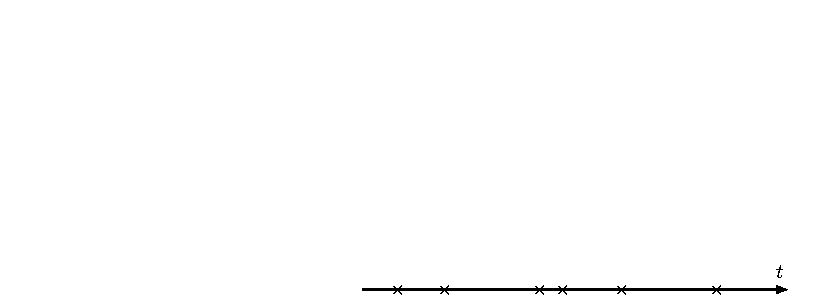
\includegraphics{images/2dpp}
\caption{فرآیند پواسن یک‌بُعدی}
\label{fig:2dpp}
\end{figure}

\section{تعریف فرآیند پواسن}
\begin{figure}
\center
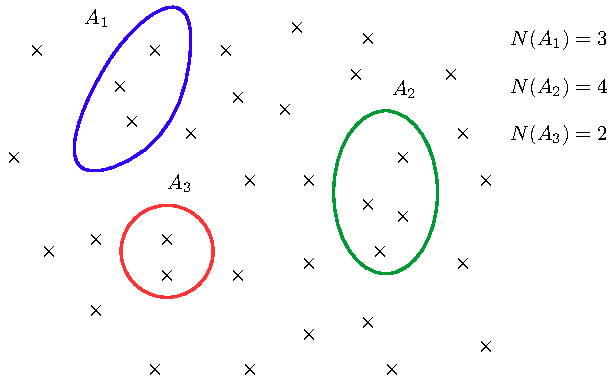
\includegraphics{images/poiss-process}
\caption{فرآیند پواسن چند‌بُعدی، استقلال آماری در توزیع نقاط}
\label{fig:ndpp}
\end{figure}
برای تعریف فرآیندهای تصادفی دو دیدگاه وجود دارد؛ مجموعه متغیرهای تصادفی و تابع تصادفی. برای تعریف فرآیند تصادفی ابتدا متغیر تصادفی را تعریف می‌کنیم \cite{williams1991probability}.
\begin{definition}%[ویلیامز \cite{williams1991probability}]
متغیر تصادفی $X$ تابعی اندازه‌پذیر از فضای احتمال $(\Omega,\mathcal{F},P)$ به  
\trans{فضای اندازه‌پذیر}{Measurable Space} $(\Xi,\mathcal{E})$
 است‌ بدین معنا که نگاشت معکوس $E\in\mathcal{E}$ عضو $\mathcal{F}$ است، $X^{-1}(E) \in \mathcal{F}$. برای تعریف توزیع احتمال متغیر تصادفی، فضای اندازه پذیر را $(\mathbb{R}, \mathcal{B}(\mathbb{R}))$ در نظر می‌گیرند\footnote{
مجموعه  $\mathcal{B}(\mathbb{R})$ از کامل کردن  $\{(-\infty,q)|q\in\mathbb{Q}\}$ به دست می‌آید، یعنی کوچکترین میدان سیگمایی که مجموعه   نیم‌باز‌ه‌های کسری عضو آن باشند.
}.
 اکنون توزیع تجمعی را می‌توان به صورت 
$F_X(x)=P(X^{-1}(-\infty,x])=P(\{\omega|X(\omega)\leq x\})$
 نوشت.
\end{definition}
از اینجا به بعد فرض می‌کنیم  فضای احتمال $(\Omega,\mathcal{F},P)$  را در اختیار داریم که همه متغیرهای تصادفی در آن قابل تعریف هستند.  اکنون تعریف فرآیند تصادفی به صورت مجموعه‌ای از متغیرهای تصادفی را می‌توان بیان کرد \cite{shalizialmost}.
\begin{definition}%[شالیزی \cite{shalizialmost}]
فرآیند تصادفی  $\{X_t\}_{t\in \mathcal{T}}$ مجموعه‌ای از متغیرهای تصادفی $X_t$ از فضای احتمال $(\Omega,\mathcal{F},P)$  به فضای اندازه‌پذیر $(\Xi,\mathcal{E})$ است‌ که با مجموعه‌ $\mathcal{T}$ نمایه می‌شوند.	
\end{definition}
برای بیان تعریف دوم، باید ابتدا تابع تصادفی و 
\trans{نمونه مسیر}{Sample path}
 را تعریف ‌کنیم \cite{shalizialmost}.

